\chapter{Algnment Examples}\label{appendix-a}

I would like to shortly compare the  alignments computed by eflomal and SimAlign with my annotations from the gold standard, especially regarding some of the examples I mentioned in Section~\ref{sec:gold-standard-examples} for handling ambiguous cases.

I will consider the following cases, which I have discussed in Section~\ref{sec:gold-standard-examples}: double negation, German preterit and perfect vs.~Romansh perfect and composite words.

In all of the examples below, filled green squares are the gold standard, circels are alignments produced by SimAlign and boxes are alignments produced eflomal.

Figure~\ref{fig:alignment-perfect} shows an example for aligning the German perfect with the Romansh perfect. 
The German and the Romansh auxiliaries \emph{hat} and \emph{ha} should be aligned to each other, as well as the German and the Romansh participles \emph{verabschiedet} and \emph{deliberà}. 
SimAlign's alignment are in accord with the gold standard, while eflomal aligned Romansh \emph{deliberà} to German \emph{hat}, leaving German \emph{verabschiedet} unaligned. However, in another case (Figure \ref{fig:alignment-perfect2}), eflomal correctly aligned the participle to the participle, and SimAlign didn't. 
It would be interesting to test this on a larger scale and see which system is more consistent regarding this.

\begin{figure}[ht]
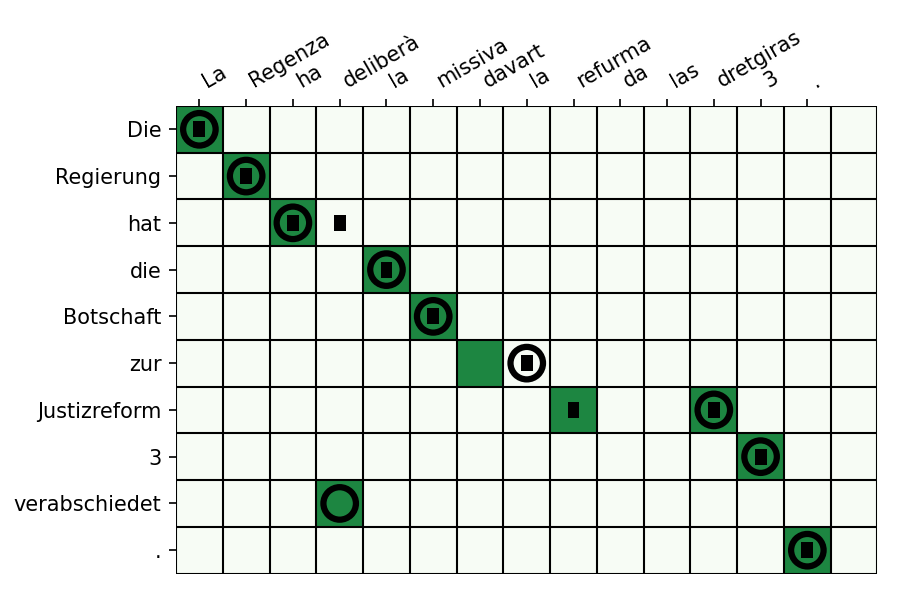
\includegraphics{graphics/alignments/example1.png}
\caption{Word alignment example for the case of perfect tense in German and Romansh}\label{fig:alignment-perfect}
\end{figure}

\begin{figure}[ht]
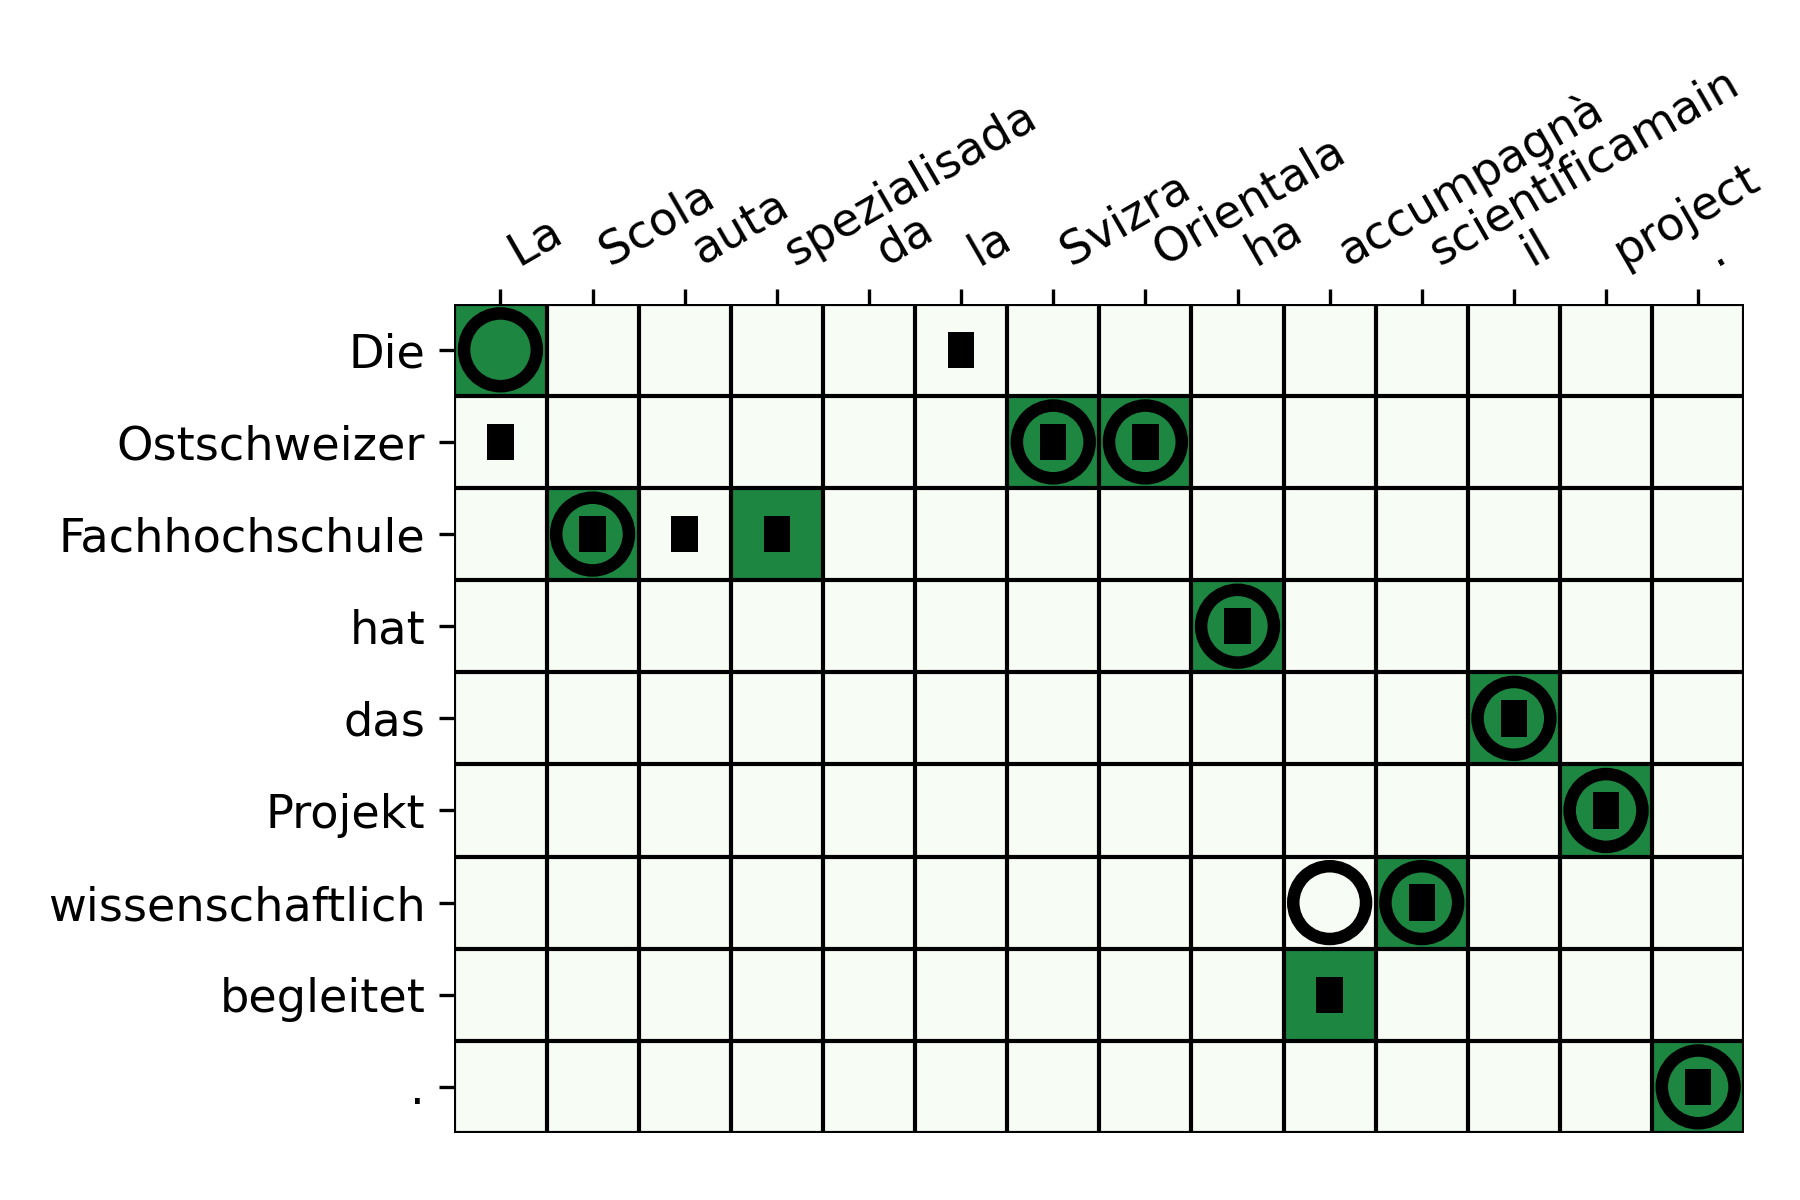
\includegraphics{graphics/alignments/example7-prefect2.png}
\caption{Word alignment example for the case of perfect tense in German and Romansh}\label{fig:alignment-perfect2}
\end{figure}





In the matter of aligning the German preterite with Romansh perfect, eflomal creates a 1-to-2 alignment, connecting both the auxiliary \emph{han} and the participle \emph{visità} to the German preterite \emph{besichtigten} (Example~\ref{fig:pret1}), an alignment which is not even acceptable, but also desirable, and which I chose to avoid in my annotations. However, in a different case, eflomal failed to align the participle, which is lexically the more important part, and left it unaligned (Example~\ref{fig:pret2}). 
SimAlign successfully aligns the German preterite to the Romansh participle in the first case, but fails as well in the second case.


\begin{figure}[ht]
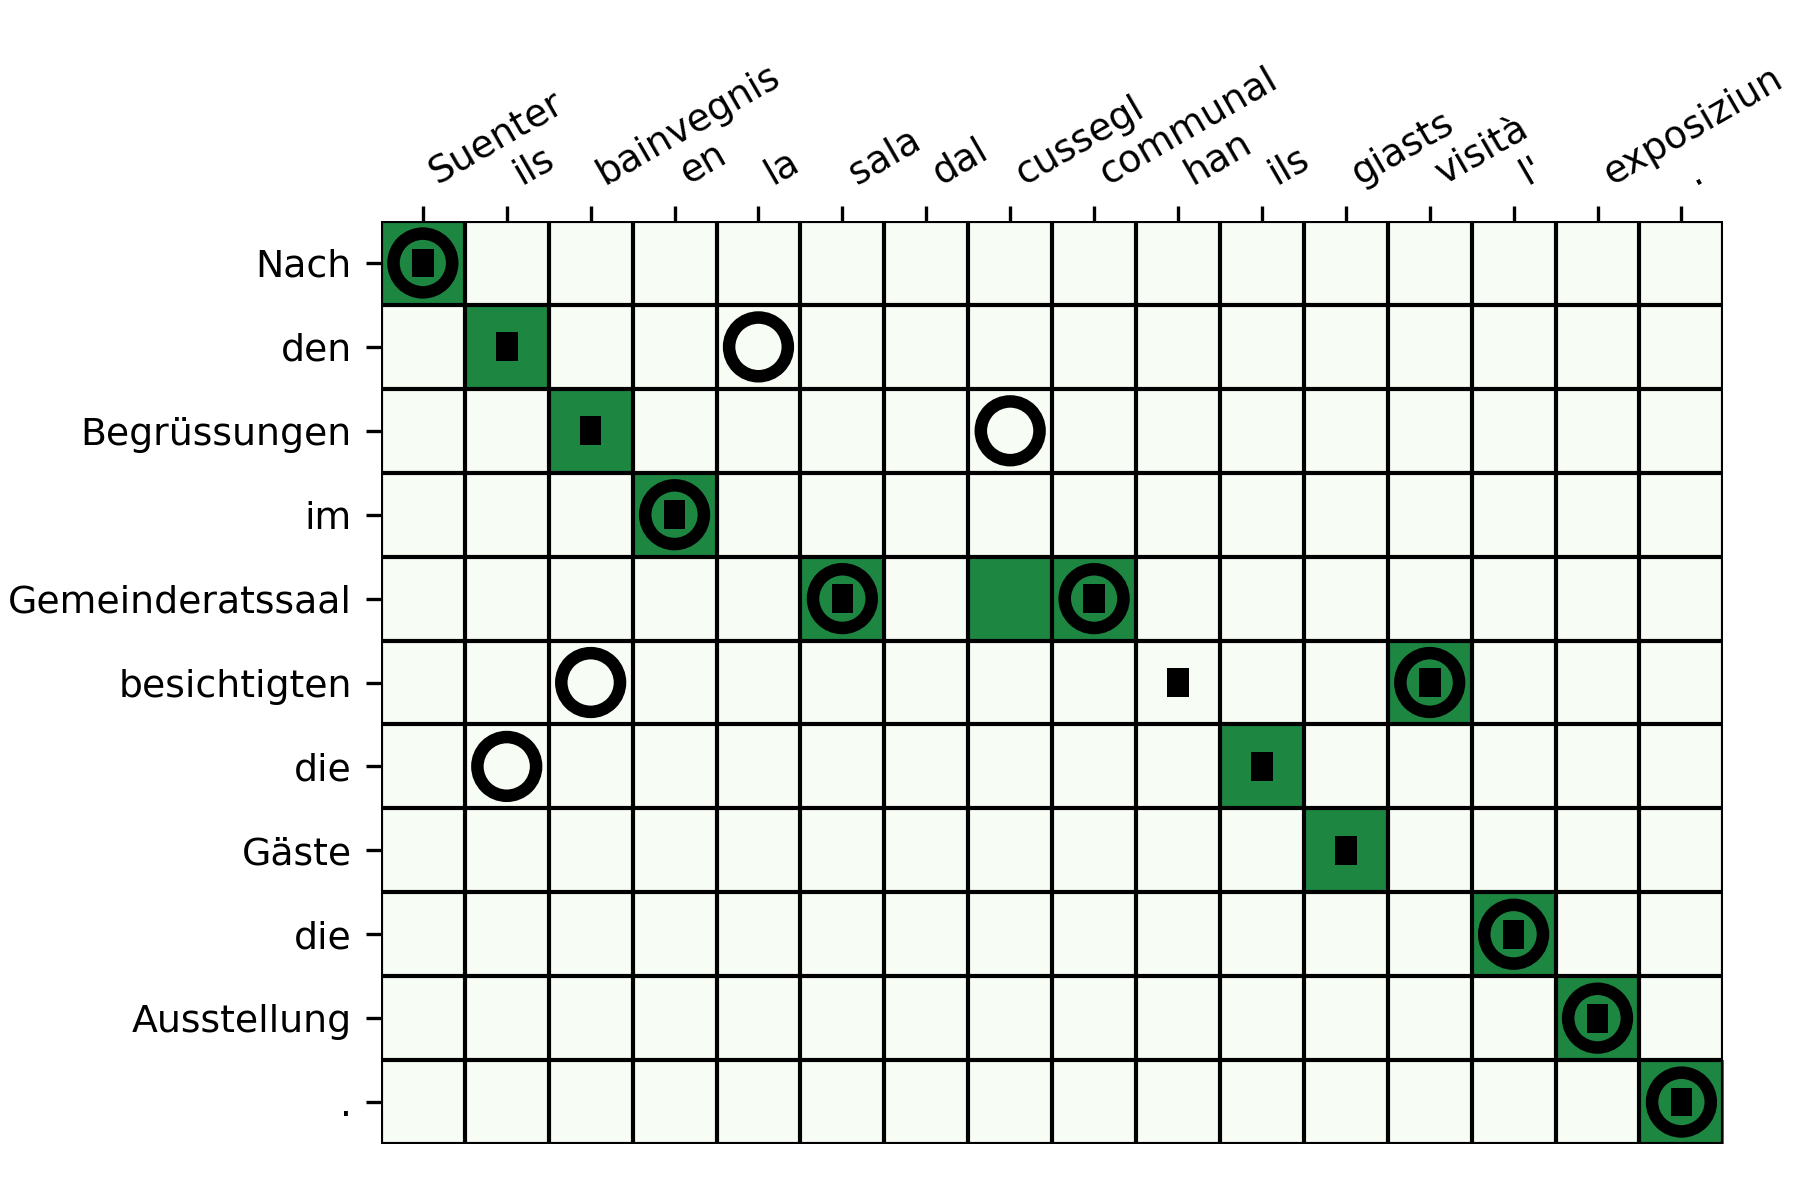
\includegraphics{graphics/alignments/example3.png}
\caption{Word alignment example for the case of German preterite}\label{fig:pret1}
\end{figure}

\begin{figure}[ht]
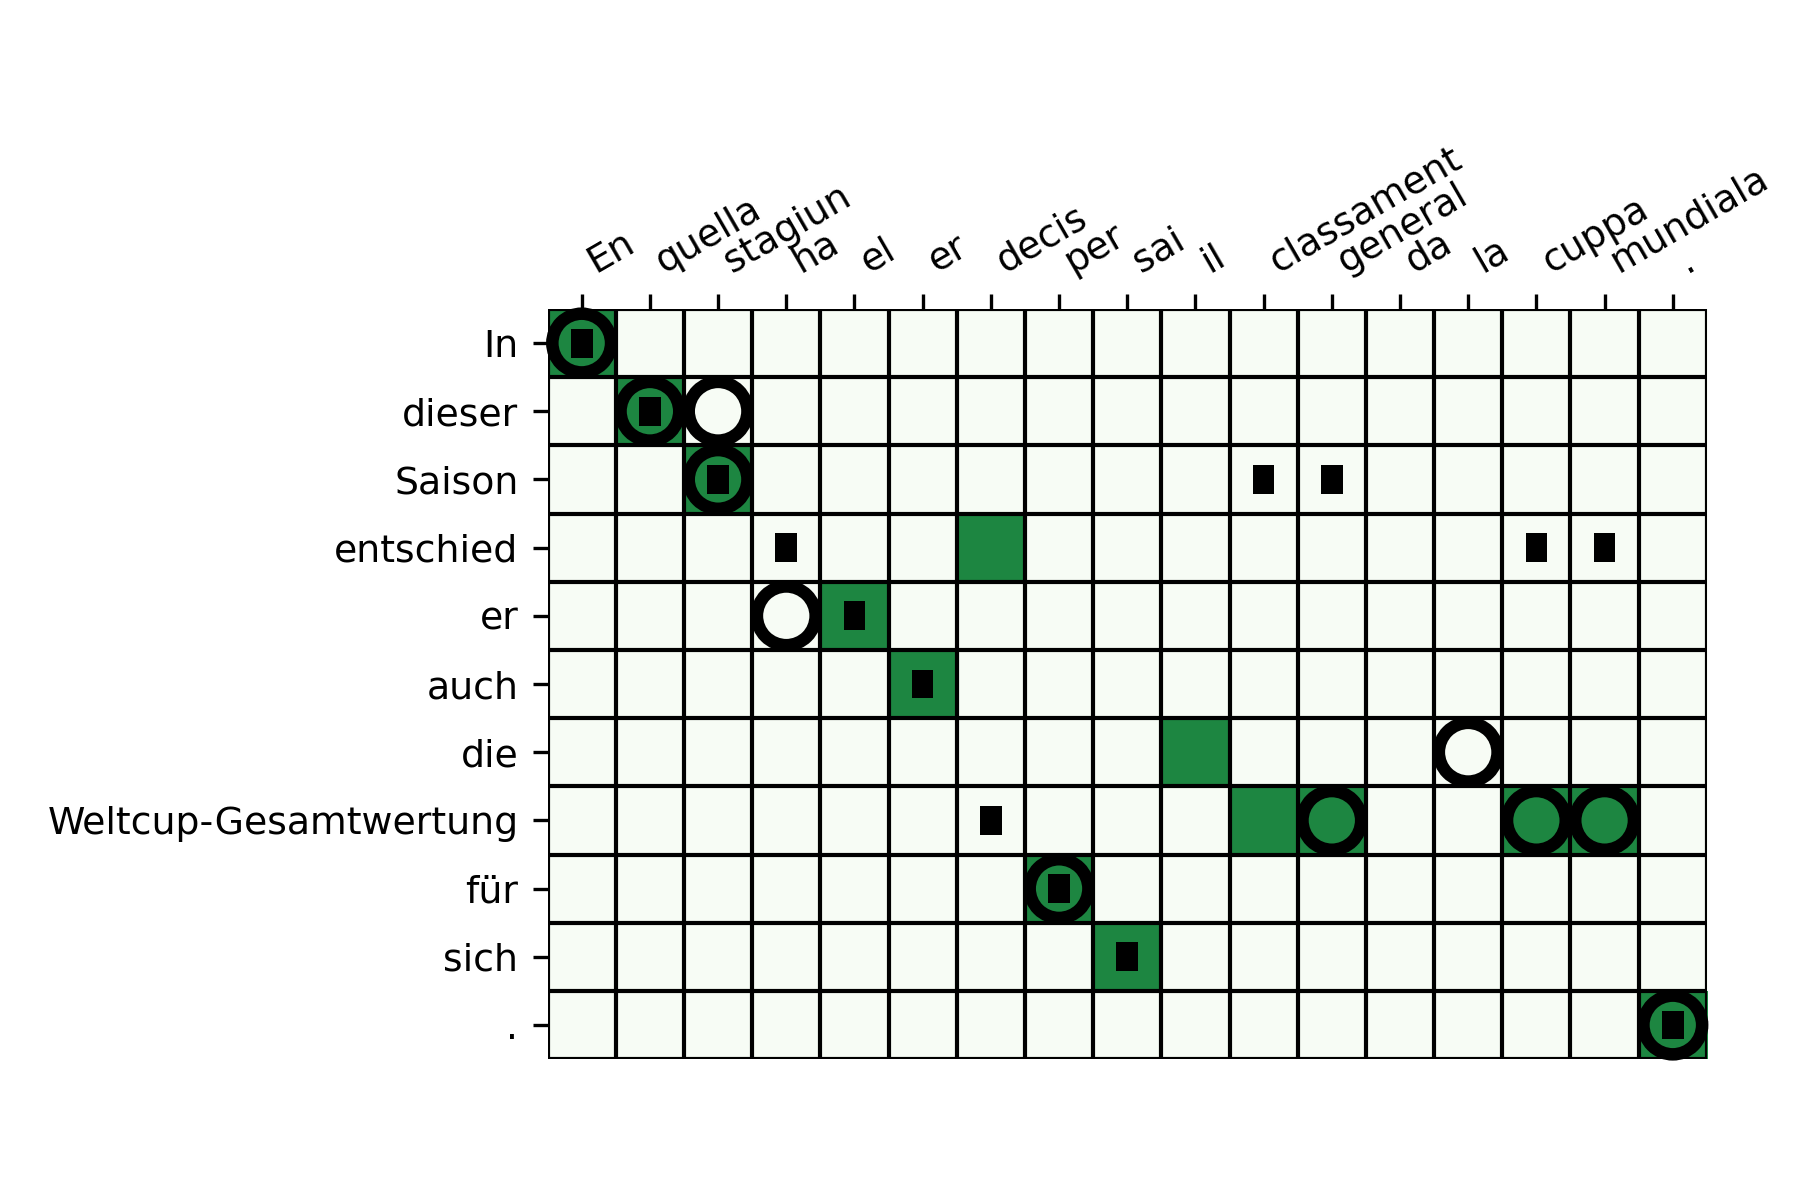
\includegraphics{graphics/alignments/example-pret.png}
\caption{Word alignment example for the case of German preterite}\label{fig:pret2}
\end{figure}






\begin{figure}[ht]
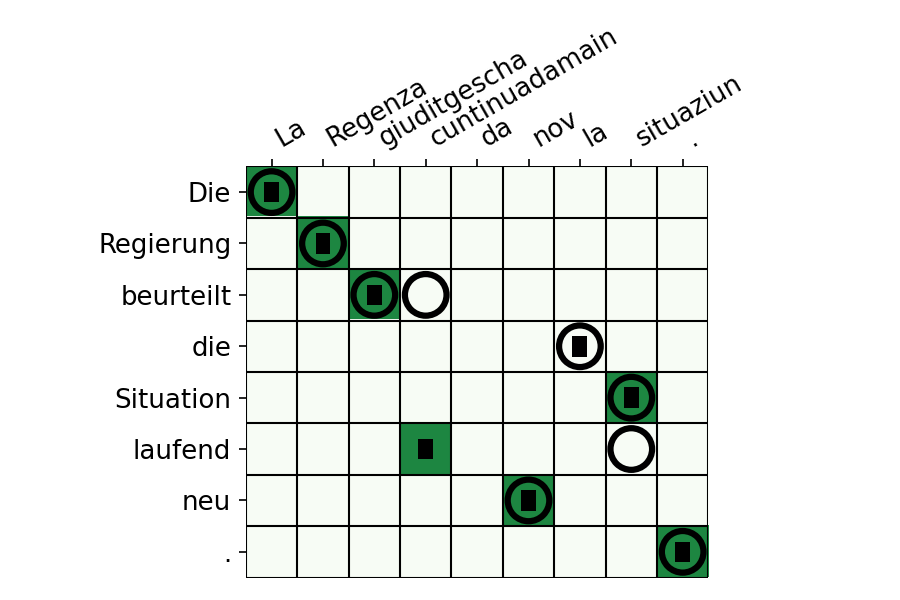
\includegraphics{graphics/alignments/example2.png}
\caption{Word alignment example 2}
\end{figure}

\begin{figure}[ht]
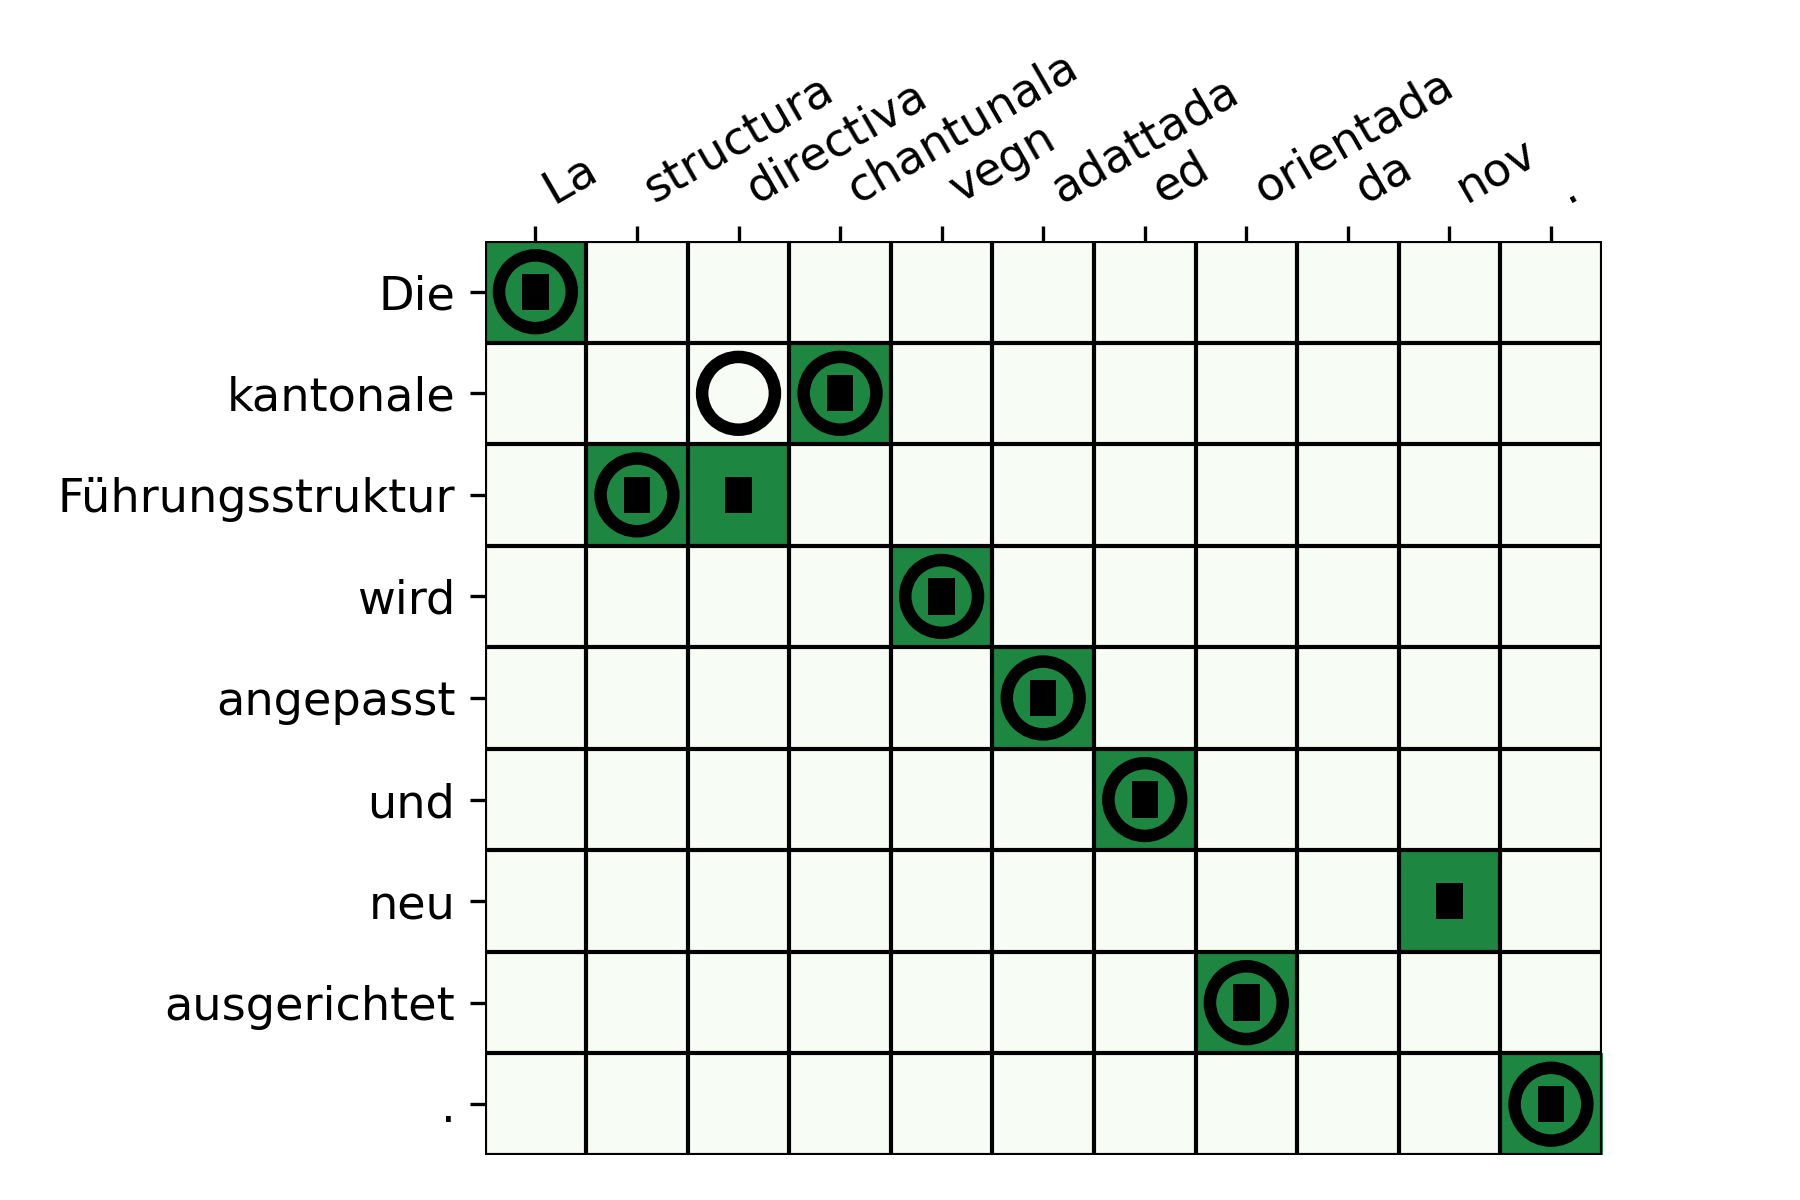
\includegraphics{graphics/alignments/example4.png}
\caption{Word alignment example 4}
\end{figure}

\begin{figure}[ht]
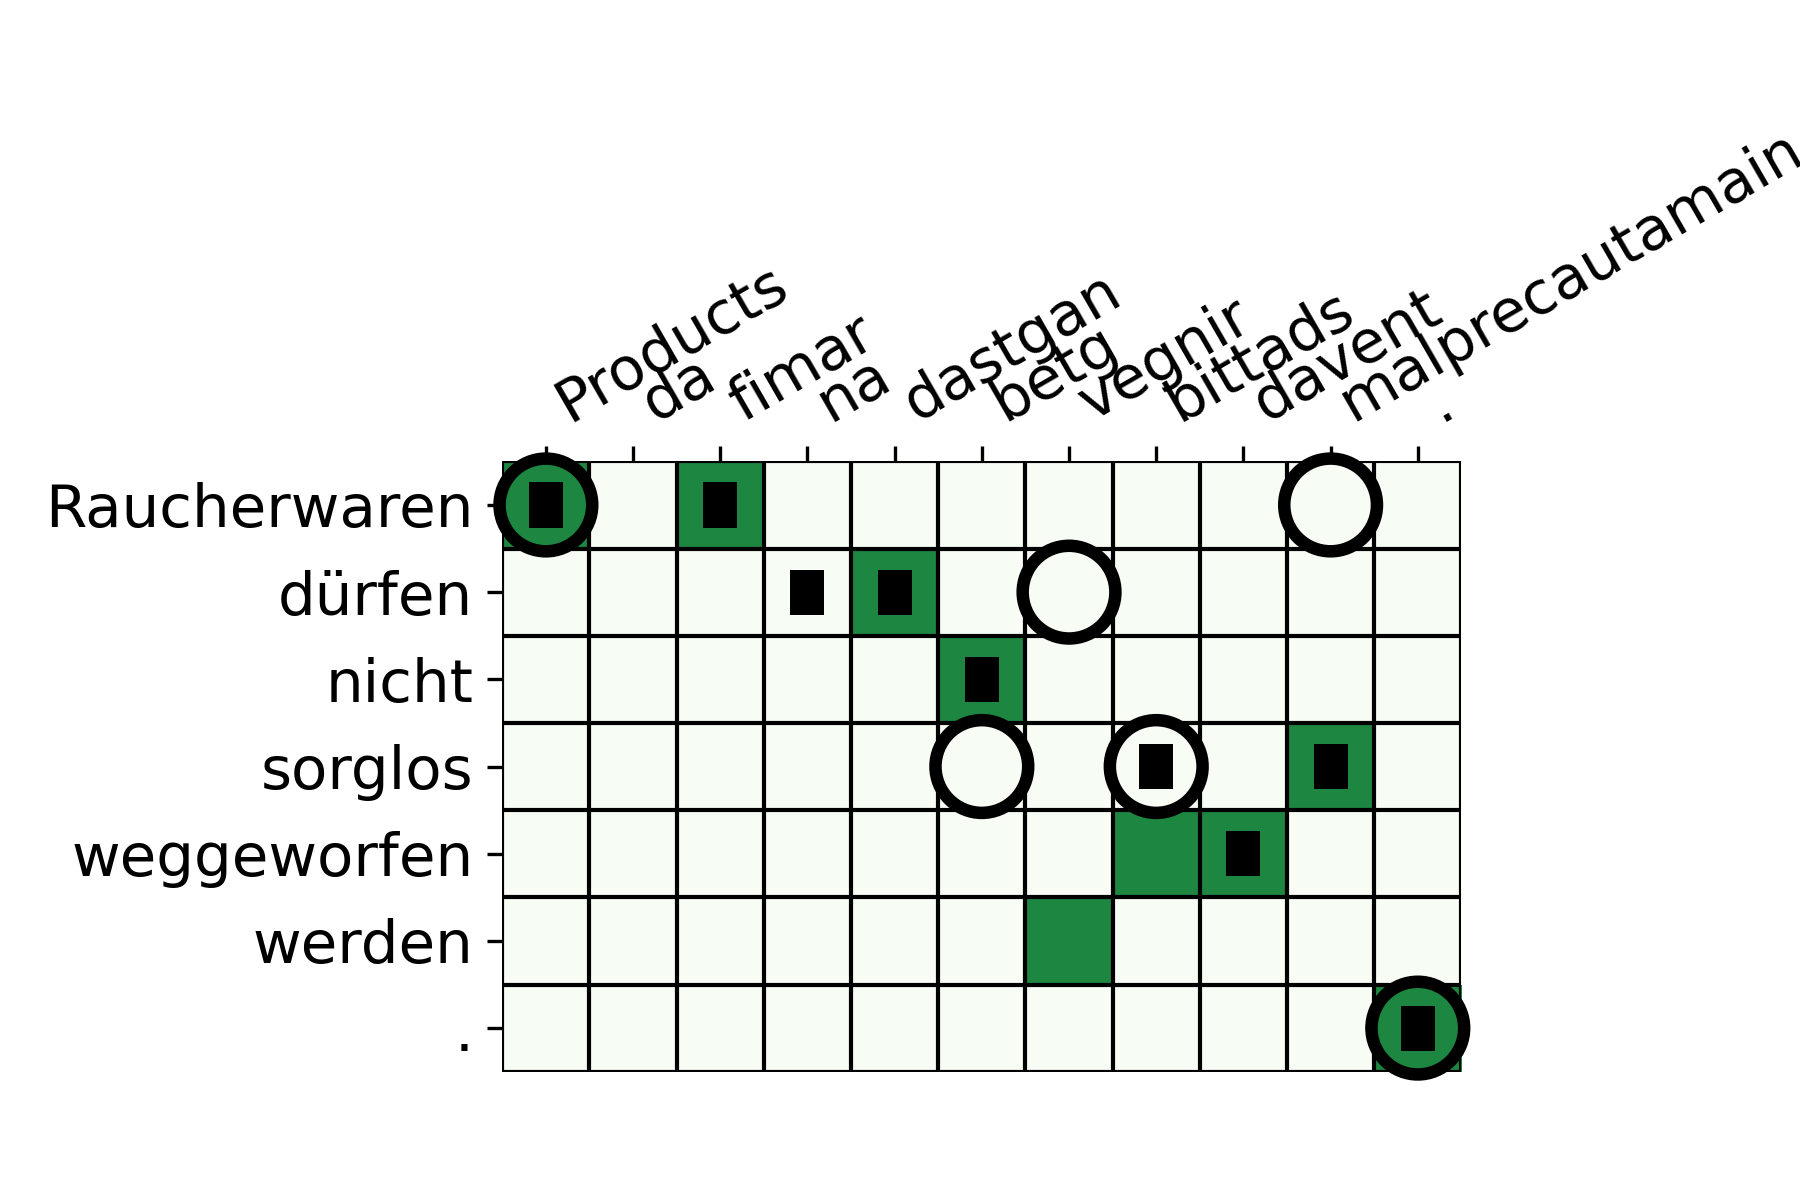
\includegraphics{graphics/alignments/example5.png}
\caption{Word alignment example 5}
\end{figure}